\section{Results}
Results for the beam-helicity and beam-charge asymmetry amplitudes extracted separately from previously published 1996-2005 and the new 2006-2007 hydrogen data sets, are presented in Figs. \ref{release_bsa_0607} and \ref{release_bca_0607}. Each of the asymmetry amplitudes is shown extracted in one bin over all kinematic variables (``overall'') and also projected against $-t$, $x_{\textrm{B}}$ and $Q^{2}$. All of the extracted asymmetry amplitudes are subject to a fractional contribution to the event yield from associated production (``Assoc. fraction''), which is shown in the bottom row of each figure. The beam-helicity asymmetry amplitudes are subject to an additional scale uncertainty from the measurement of the beam polarisation, which is stated in the captions of the figures.
\begin{figure}
\begin{center}
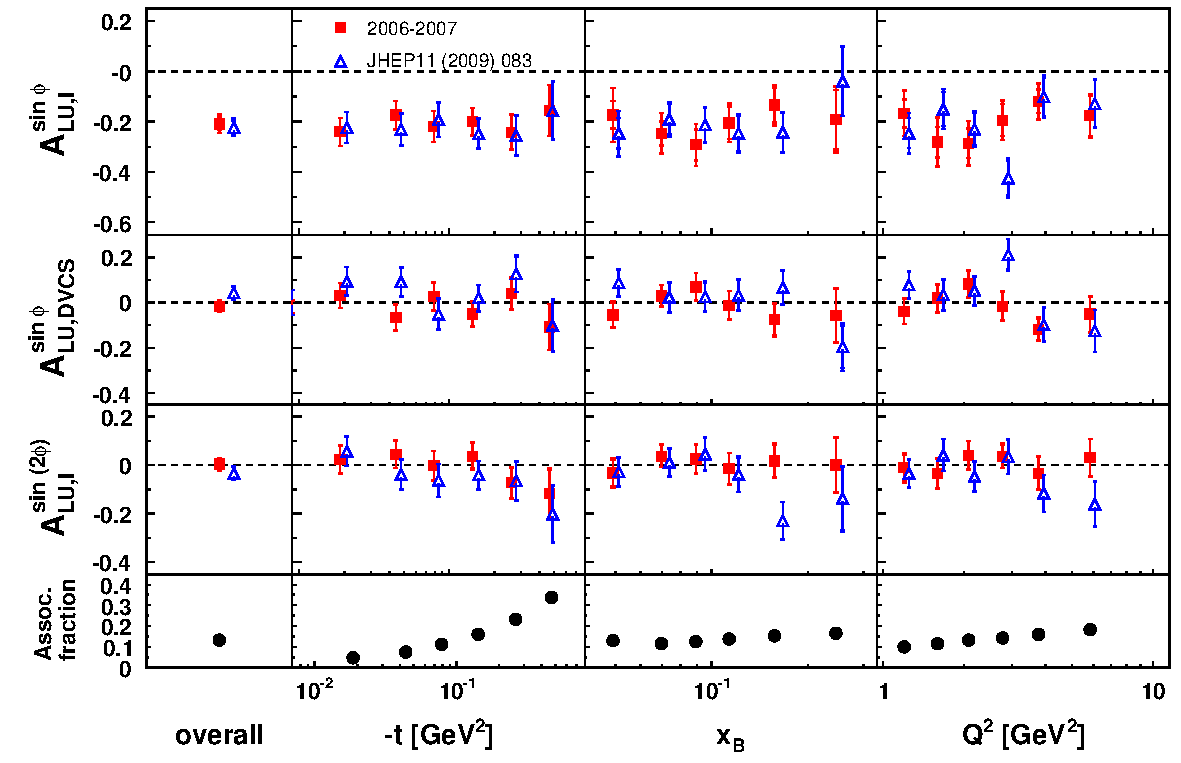
\includegraphics[width=15cm,keepaspectratio]{bsadvcsplots_eml_par13_bin6_release_pic_update_0607_9605}
  \caption{Beam-helicity asymmetry amplitudes extracted separately from
the 1996-2005 (open triangles) and 2006-2007 (filled squares)
hydrogen data. The inner error bars represent the statistical uncertainties, while total error bars denote the statistical and systematic uncertainties added in quadrature.  
An additional 2.8\,\% and 3.4\,\% scale uncertainty for the 1996-2005 and
2006-2007 data respectively is present in the amplitudes due to the imprecision of
the beam polarisation measurement. The simulated fractional contribution from associated production to the yield in each kinematic bin is shown in the bottom row.}
 \label{release_bsa_0607}
\end{center}
 \end{figure}

A statistical test was applied in order to check for possible incompatibility between the asymmetry amplitudes extracted from both data sets. Only the statistical uncertainties were employed in this test. \blue{This test revealed no significant evidence for incompatibility between the data sets.} The \blue{beam-helicity and beam-charge} asymmetry amplitudes can therefore be extracted from the complete hydrogen data set recorded during the entire experimental operation of H{\sc ermes}.
\begin{figure}
\begin{center}
 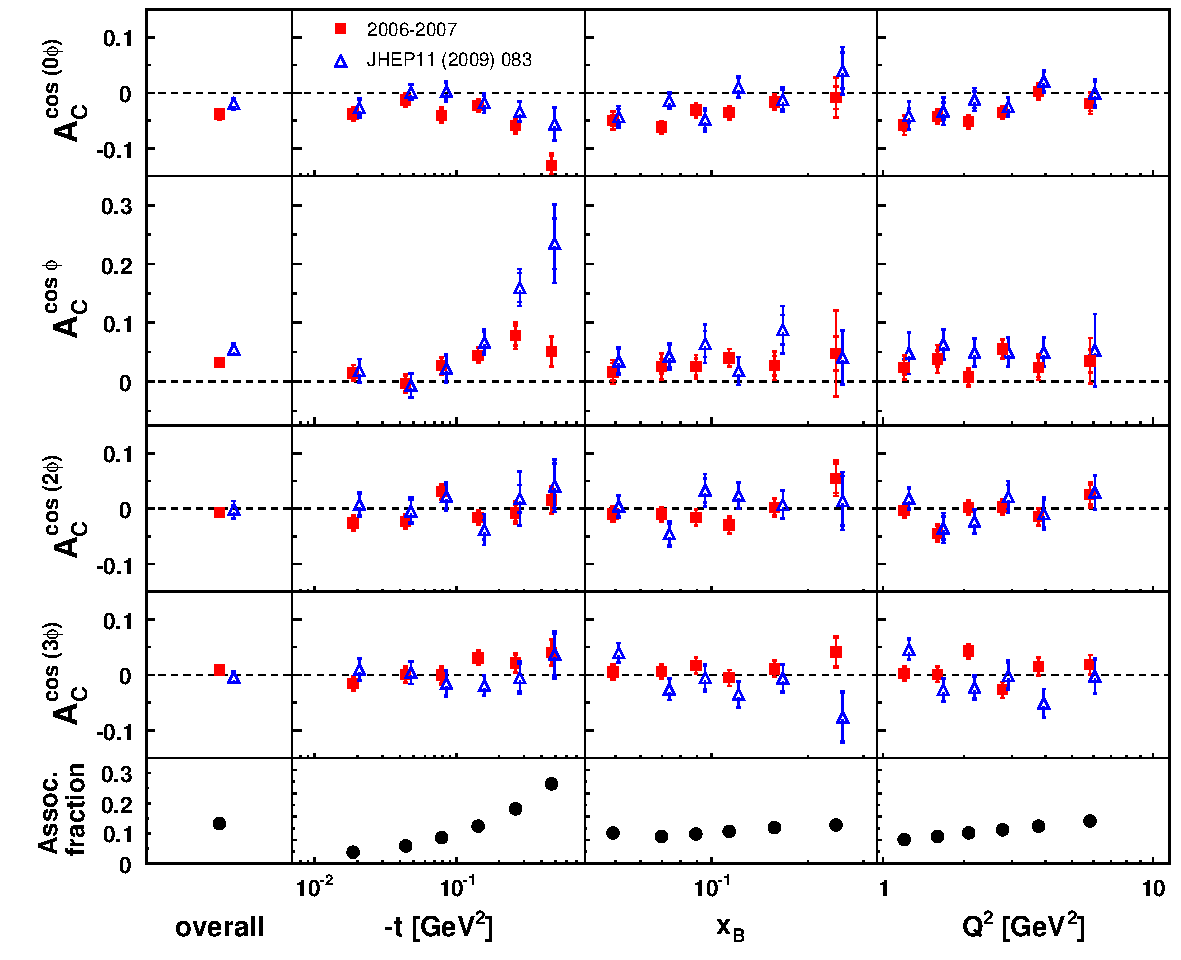
\includegraphics[width=15cm,keepaspectratio]{bcaplots_eml_par13_bin6_release_pic_update_0607_9605_withassoc}
  \caption{Beam-charge asymmetry amplitudes extracted separately from the 1996-2005 (open triangles) and 2006-2007 (filled squares) hydrogen data.
The inner error bars represent the statistical uncertainties, while the total error bars denote the statistical and systematic uncertainties added in quadrature. The simulated fractional contribution from associated production to the yield in each kinematic bin is shown in the bottom row.}
 \label{release_bca_0607}
\end{center}
 \end{figure}

\begin{figure}
 \begin{center}
 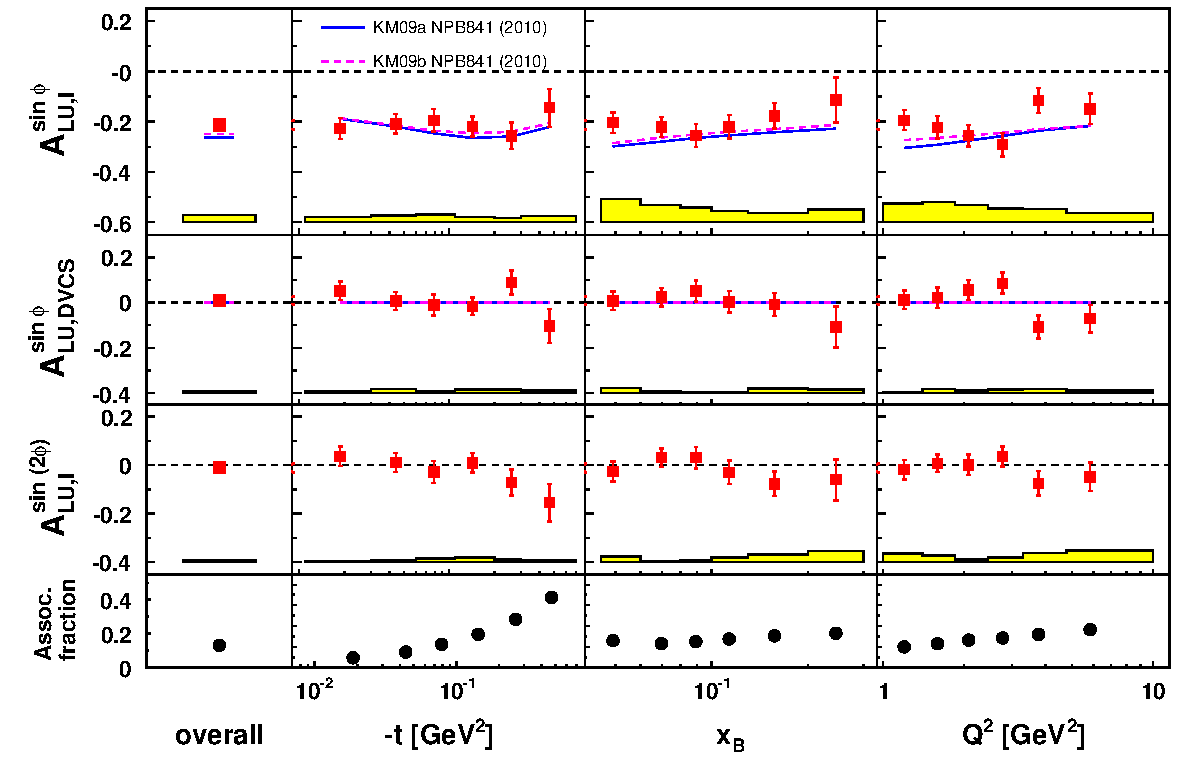
\includegraphics[width=15cm]{bsadvcsplots_eml_par13_bin6_release_all_pic_update}
  \caption{The $A_{\textrm{LU,I}}^{\sin\phi}$, $A_{\textrm{LU,DVCS}}^{\sin\phi}$ and
$A_{\textrm{LU,I}}^{\sin(2\phi)}$ beam-helicity asymmetry amplitudes extracted from all the hydrogen data recorded at H{\sc ermes}
from 1996 until 2007. The error bars (bands) represent the statistical
(systematic) uncertainties. An additional 3.2\,\% scale uncertainty is present in the amplitudes due to the imprecision of
the beam polarisation measurement. Theoretical calculations from the model described in \blue{Ref.} \cite{Kum09} are shown as solid and dashed lines. See text for details. The simulated fractional contribution from associated production to the yield in each kinematic bin is shown in the bottom row.}
  \label{bsa_xbjrange}
 \end{center}
\end{figure}

\begin{figure}
  \begin{center}
    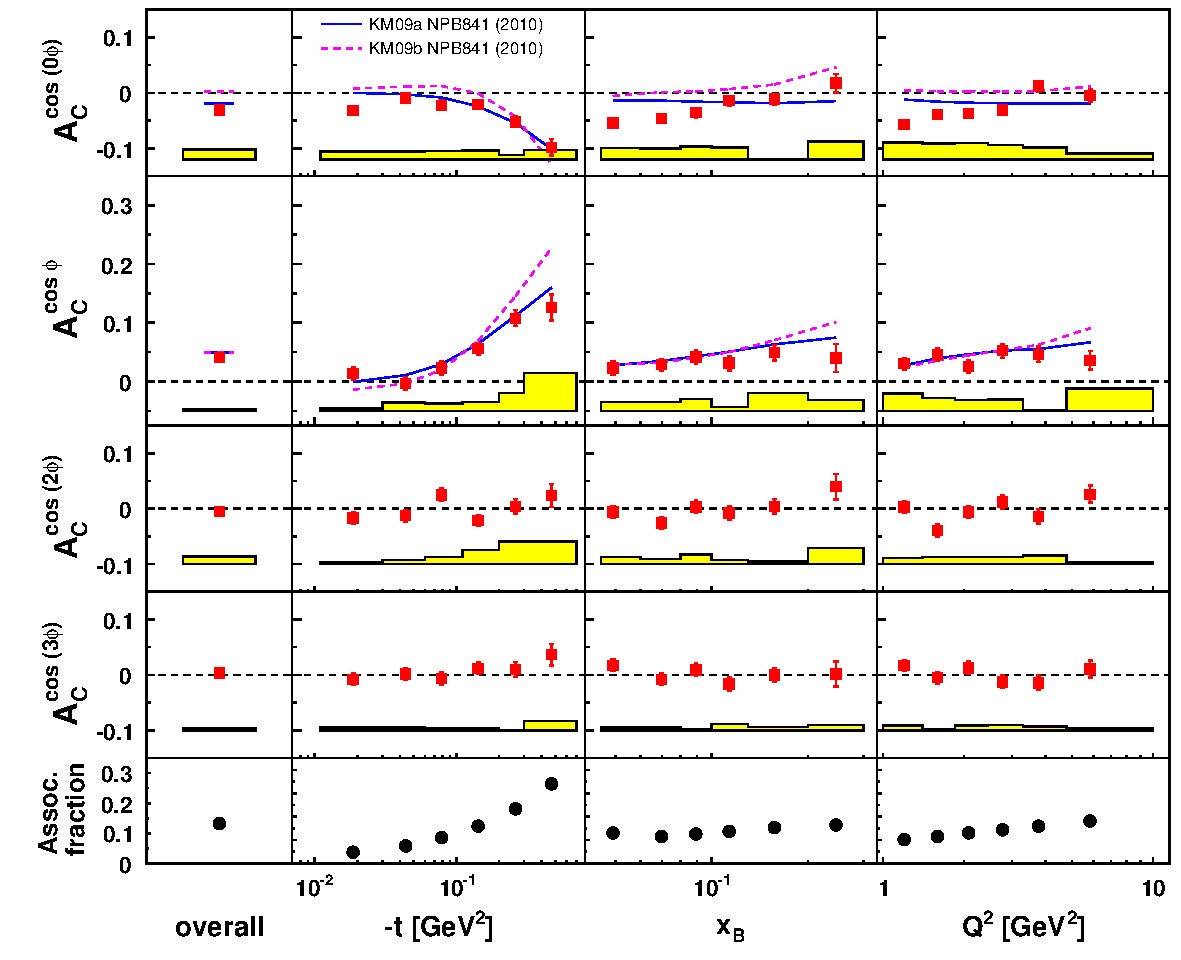
\includegraphics[width=15cm]{bcaplots_eml_par13_bin6_all_release_pic_update_withassoc}
    \caption{The $A_{\textrm{C}}^{\cos(0\phi)}$, $A_{\textrm{C}}^{\cos\phi}$, $A_{\textrm{C}}^{\cos(2\phi)}$ and $A_{\textrm{C}}^{\cos(3\phi)}$ beam-charge asymmetry amplitudes extracted from all the hydrogen data recorded at H{\sc ermes} from 1996 until 2007. The error bars (bands) represent the statistical (systematic) uncertainties.  Theoretical calculations from the model described in \blue{Ref.} \cite{Kum09} are shown as solid and dashed lines. See text for details. The simulated fractional contribution from associated production to the yield in each kinematic bin is shown in the bottom row.}
  \label{bca_xbjrange}
 \end{center}
\end{figure}

\begin{figure}
 \begin{center}
 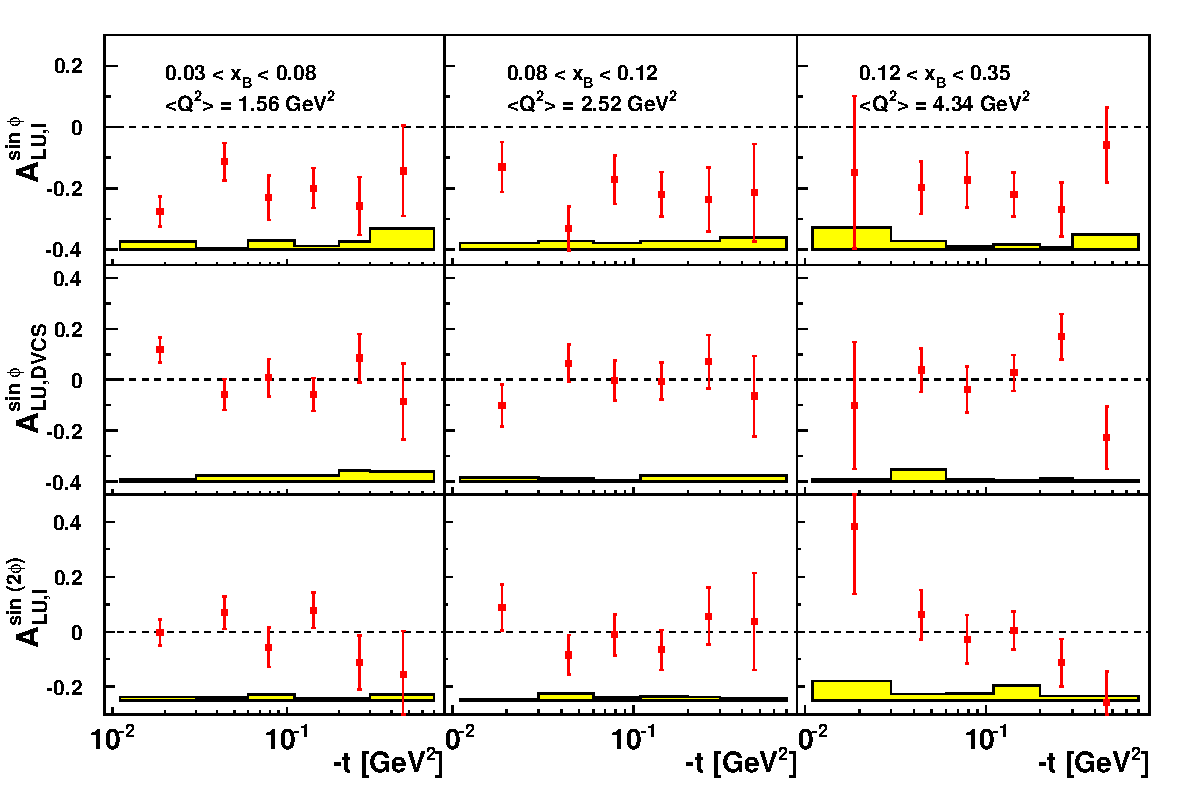
\includegraphics[width=15cm]{bsadvcsplots_tc_xbjrange_eml_par13_bin6_9607_pic_update}
  \caption{The $A_{\textrm{LU,I}}^{\sin\phi}$, $A_{\textrm{LU,DVCS}}^{\sin\phi}$ and
$A_{\textrm{LU,I}}^{\sin(2\phi)}$ beam-helicity asymmetry amplitudes extracted from all the hydrogen data recorded at H{\sc ermes}
from 1996 until 2007 as a function of $-t$ for three different $x_{\textrm{B}}$ ranges. The error bars (bands) represent the statistical
(systematic) uncertainties. An additional 3.2\,\% scale uncertainty is present in the amplitudes due to the imprecision of
the beam polarisation measurement.}
  \label{bsa_xbjrange2}
 \end{center}
\end{figure}

\begin{figure}
  \begin{center}
    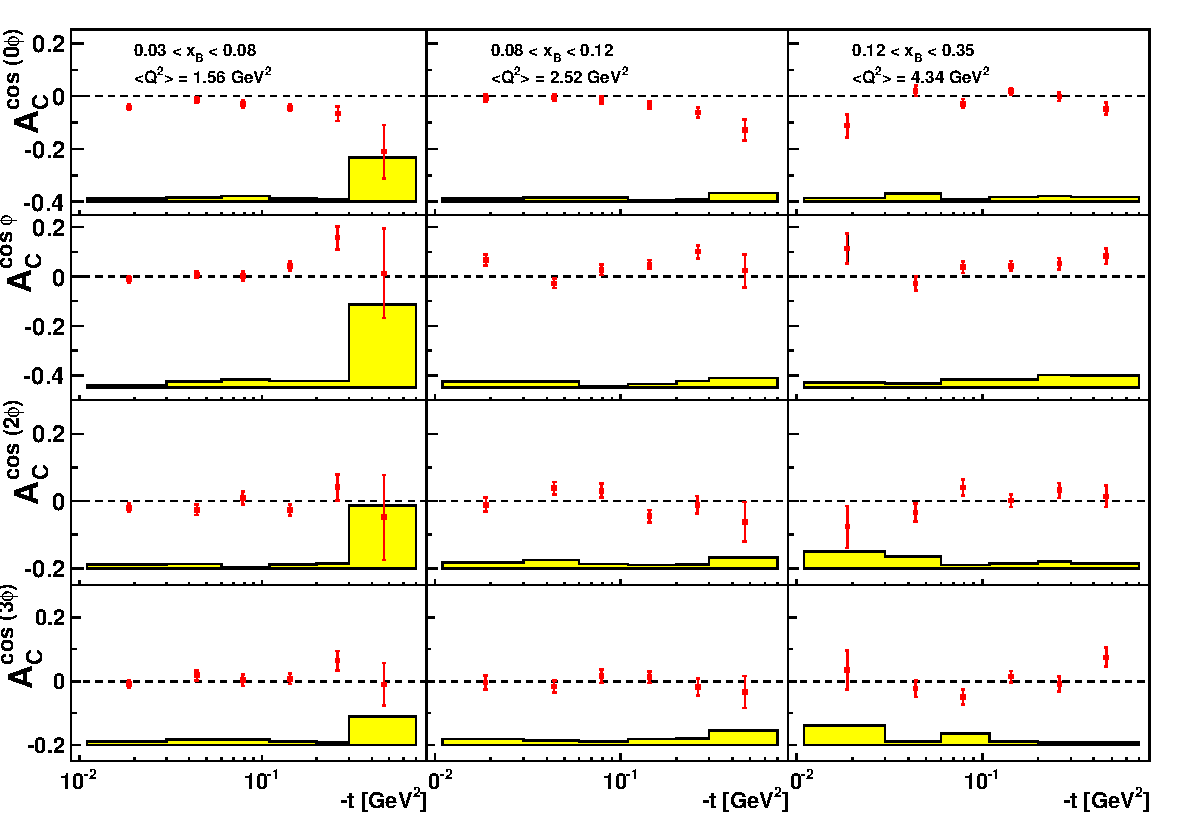
\includegraphics[width=15cm]{bcaplots_tc_xnjrange_eml_par13_bin6_9607_pic}
    \caption{The $A_{\textrm{C}}^{\cos(0\phi)}$, $A_{\textrm{C}}^{\cos\phi}$, $A_{\textrm{C}}^{\cos(2\phi)}$ and $A_{\textrm{C}}^{\cos(3\phi)}$ beam-charge asymmetry amplitudes extracted from all the hydrogen data recorded at H{\sc ermes} from 1996 until 2007 as a function of $-t$ for three different $x_{\textrm{B}}$ ranges. The error bars (bands) represent the statistical (systematic) uncertainties.}
  \label{bca_xbjrange2}
 \end{center}
\end{figure}

The results of the beam-helicity and beam-charge asymmetry amplitudes extracted from the complete 1996-2007 hydrogen sample are shown in Figs.~\ref{bsa_xbjrange} and \ref{bca_xbjrange}. The number of analysable events available from the 2006-2007 data set (67815) is approximately three times greater than the number of events recorded in the 1996-2005 sample (24817). The  asymmetry amplitudes extracted from the complete 1996-2007 data set are thus weighted towards the 2006-2007 result. This weighting towards the 2006-2007 result is not so evident for the beam helicity asymmetry amplitudes because the beam polarisation was lower in 2006 and 2007.

The first and second harmonics of $\mathcal{A}_{\textrm{LU,I}}$, which are
sensitive to the interference term in the scattering amplitude, \blue{is} shown in the first and third rows of Fig.~\ref{bsa_xbjrange}. The leading-twist amplitude $A_{\textrm{LU,I}}^{\sin\phi}$ has the largest value of any of the amplitudes when extracted in a single bin from the entire data set. This amplitude has no strong dependence on $-t$, $x_{\textrm{B}}$ or $Q^{2}$, implying a strong dependence at smaller values of $-t$ as the amplitude must diminish in this $-t$ region due to the dependence of the amplitude on the factor $k$ from Eq.~\ref{eq:s1}. The $A_{\textrm{LU,I}}^{\sin\phi}$ amplitude is sensitive to the imaginary part of the CFF $\mathcal{H}$ and thereby can constrain GPD $\textit{H}$. The twist-3 $A_{\textrm{LU,I}}^{\sin(2\phi)}$ amplitude is compatible with zero, as is the twist-3 $A_{\textrm{LU,DVCS}}^{\sin\phi}$ amplitude, which is dependent on the squared DVCS term. The $A_{\textrm{LU,DVCS}}^{\sin\phi}$ amplitude are shown in the second row of Fig.~\ref{bsa_xbjrange}. Neither the $A_{\textrm{LU,DVCS}}^{\sin\phi}$ nor the $A_{\textrm{LU,I}}^{\sin(2\phi)}$ amplitude show any clear dependence on $-t$, $x_{\textrm{B}}$ or $Q^{2}$. The systematic error bands associated with the asymmetry amplitudes extracted from the combined data set were determined using Monte Carlo simulations that reflect the equipment used in the various stages of the H{\sc ermes} experiment. 

The $A_{\textrm{C}}^{\cos(n\phi)}$ amplitudes are shown in Fig.~\ref{bca_xbjrange}. The leading-twist $A_{\textrm{C}}^{\cos(0\phi)}$ and $A_{\textrm{C}}^{\cos\phi}$ amplitudes are both non-zero. There is a relationship between $A_{\textrm{C}}^{\cos(0\phi)}$ and $A_{\textrm{C}}^{\cos\phi}$ as the Fourier coefficient $c^{\textrm{I}}_{0,\textrm{unp}}$ is inversely proportional to $c^{\textrm{I}}_{1,\textrm{unp}}$ via the kinematic factor $k$ from Eq.~\ref{eq:c1}. These amplitudes diverge with opposite sign from zero at increasing values of $-t$ but they
have no discernible dependence on $x_{\textrm{B}}$ and $Q^{2}$. The $A_{\textrm{C}}^{\cos(2\phi)}$ and $A_{\textrm{C}}^{\cos(3\phi)}$ amplitudes are both consistent with zero and have no significant variation in value over the range in $-t$, $x_{\textrm{B}}$ and $Q^{2}$. The $A_{C}^{\cos(2\phi)}$ \blue{amplitude} is related to twist-3 GPDs and $A_{\textrm{C}}^{\cos(3\phi)}$ relates to gluon helicity-flip GPDs. Both of these amplitudes are expected to be suppressed at H{\sc ermes} kinematic conditions compared to the leading\blue{-}twist amplitudes.

The curves in Figs.~\ref{bsa_xbjrange} and~\ref{bca_xbjrange} show calculations from a global fit of GPDs to experimental data~\cite{Kum09}. The basic model is a minimalist dual representation of GPDs with only (very) weakly entangled skewness and $t$ dependences. In the model, the $t$ dependence is approximated by a physically-motivated Regge dependence. The solid curves represent the model fit without data from experiments \cite{Cam06, Gir08} at Hall A in Jefferson Laboratory; the model fit represented by the dashed curves includes this data. Both fits include the 1996-2005 H{\sc ermes} data. The model incorporates only twist-2 GPDs and so can provide calculations only for the $A_{\textrm{LU,I}}^{\sin\phi}$, $A_{\textrm{C}}^{\cos(0\phi)}$ and $A_{\textrm{C}}^{\cos\phi}$ asymmetry amplitudes. All of the amplitudes are well described by the model.

In order to provide more detailed information \blue{that will be used in} future fits, in particular for the determination of the entanglement of the skewness and $-t$ dependences of GPDs, the amplitudes already presented in Figs.~\ref{bsa_xbjrange} and~\ref{bca_xbjrange} are shown as a function of $-t$ for three different ranges of $x_{\textrm{B}}$ in Figs.~\ref{bsa_xbjrange2} and~\ref{bca_xbjrange2}. There is no observed $-t$ depend\blue{ence} on any of the \blue{$\mathcal{A}_{\textrm{LU}}$} amplitudes in either of the distinct ranges of $x_{\textrm{B}}$. Also no additional features or $-t$ dependenc\blue{es} are observed for the \blue{$\mathcal{A}_{\textrm{C}}$} amplitudes in these separate $x_{\textrm{B}}$ ranges.
